\documentclass[tikz,border=12pt]{standalone}
\usepackage[T1]{fontenc}
\usepackage{mathpazo}
\usepackage{amsmath,amssymb}
\usetikzlibrary{arrows.meta, calc}

\definecolor{stblue}{HTML}{7B97AD}
\definecolor{rwgold}{HTML}{B8995E}
\definecolor{sage}{HTML}{7A9A7E}
\definecolor{dkbrown}{HTML}{3D3530}
\definecolor{wmgray}{HTML}{7B7067}
\definecolor{cream}{HTML}{F9F6F0}
\definecolor{border}{HTML}{D4C9B8}
\definecolor{terracotta}{HTML}{C47A6A}
\definecolor{lavender}{HTML}{907EA0}

\begin{document}
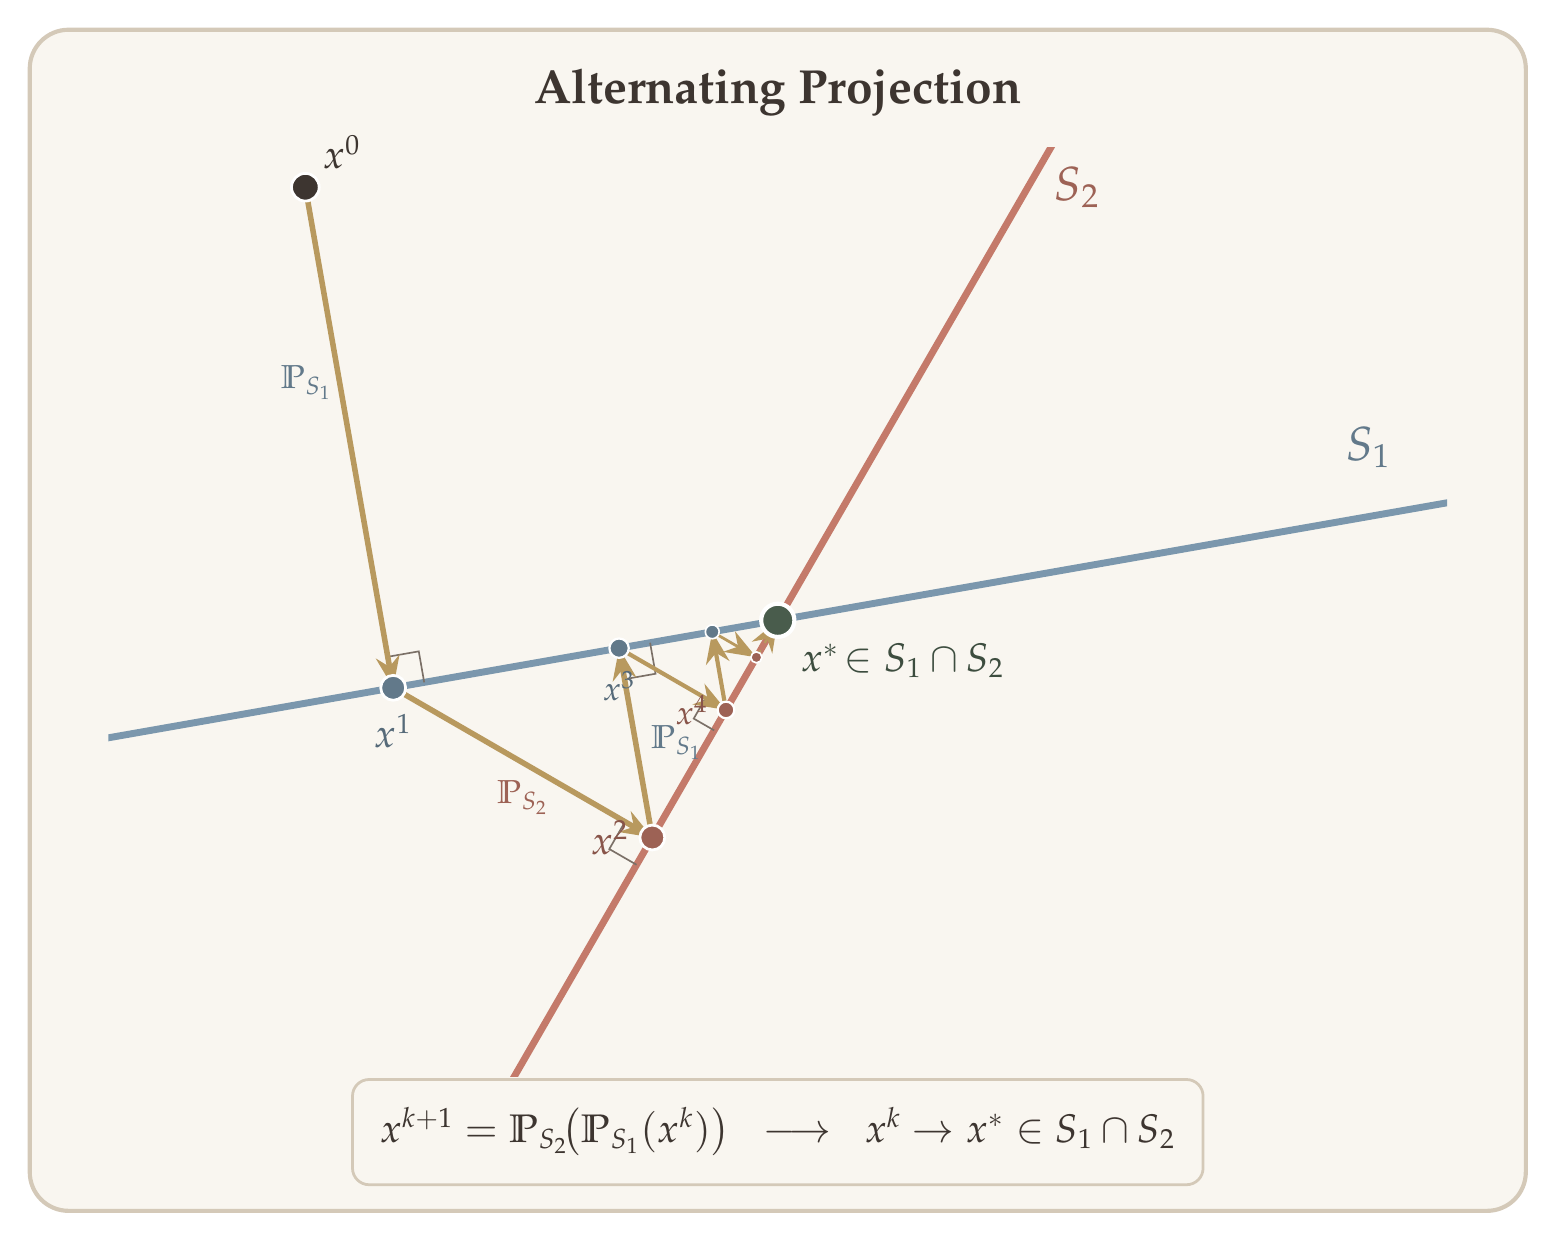
\begin{tikzpicture}[>={Stealth[length=4mm, width=3mm]}]

% Background
\fill[cream, rounded corners=14pt] (-1.5,-3.5) rectangle (17.5,11.5);
\draw[border, line width=1.5pt, rounded corners=14pt] (-1.5,-3.5) rectangle (17.5,11.5);

% Title
\node[text=dkbrown, font=\LARGE\bfseries] at (8.0,10.7)
  {Alternating Projection};

% ================================================================
% Two lines (affine subspaces) intersecting at x*
% ================================================================
% S1: through (8,4), angle ~10 deg, slope = tan(10) ~ 0.176
\coordinate (S1L) at (-1, 2.42);
\coordinate (S1R) at (17, 5.58);
% S2: through (8,4), angle ~60 deg, slope = tan(60) ~ 1.732
\coordinate (S2L) at (4.5, -2.06);
\coordinate (S2R) at (11.5, 10.06);

% Draw lines (clipped to content area)
\begin{scope}
  \clip (-0.5,-1.8) rectangle (16.5,10.0);
  \draw[stblue, line width=2.5pt] (S1L) -- (S1R);
  \draw[terracotta, line width=2.5pt] (S2L) -- (S2R);
\end{scope}

% Line labels
\node[text=stblue!80!black, font=\LARGE\bfseries] at (15.5, 6.2) {$S_1$};
\node[text=terracotta!80!black, font=\LARGE\bfseries] at (11.8, 9.5) {$S_2$};

% ================================================================
% Alternating projections (exact, computed by TikZ)
% ================================================================
\coordinate (x0) at (2.0, 9.5);

% TikZ calc: $(A)!(P)!(B)$ = orthogonal projection of P onto line AB
\coordinate (x1) at ($(S1L)!(x0)!(S1R)$);   % P_{S1}(x0)
\coordinate (x2) at ($(S2L)!(x1)!(S2R)$);   % P_{S2}(x1)
\coordinate (x3) at ($(S1L)!(x2)!(S1R)$);   % P_{S1}(x2)
\coordinate (x4) at ($(S2L)!(x3)!(S2R)$);   % P_{S2}(x3)
\coordinate (x5) at ($(S1L)!(x4)!(S1R)$);   % P_{S1}(x4)
\coordinate (x6) at ($(S2L)!(x5)!(S2R)$);   % P_{S2}(x5)

% Intersection point
\coordinate (xstar) at (8, 4);

% ================================================================
% Right-angle markers (proving projections are orthogonal)
% ================================================================
% At x1 (proj onto S1): mark between incoming direction and S1
\coordinate (m1a) at ($(x1)!4mm!(x0)$);
\coordinate (m1b) at ($(x1)!4mm!(S1R)$);
\coordinate (m1c) at ($(m1a)+(m1b)-(x1)$);
\draw[wmgray, line width=0.6pt] (m1a) -- (m1c) -- (m1b);

% At x2 (proj onto S2)
\coordinate (m2a) at ($(x2)!4mm!(x1)$);
\coordinate (m2b) at ($(x2)!4mm!(S2L)$);
\coordinate (m2c) at ($(m2a)+(m2b)-(x2)$);
\draw[wmgray, line width=0.6pt] (m2a) -- (m2c) -- (m2b);

% At x3 (proj onto S1)
\coordinate (m3a) at ($(x3)!4mm!(x2)$);
\coordinate (m3b) at ($(x3)!4mm!(S1R)$);
\coordinate (m3c) at ($(m3a)+(m3b)-(x3)$);
\draw[wmgray, line width=0.6pt] (m3a) -- (m3c) -- (m3b);

% At x4 (proj onto S2)
\coordinate (m4a) at ($(x4)!3mm!(x3)$);
\coordinate (m4b) at ($(x4)!3mm!(S2L)$);
\coordinate (m4c) at ($(m4a)+(m4b)-(x4)$);
\draw[wmgray, line width=0.6pt] (m4a) -- (m4c) -- (m4b);

% ================================================================
% Projection arrows
% ================================================================
\draw[rwgold, line width=2pt, ->] (x0) -- (x1);
\draw[rwgold, line width=2pt, ->] (x1) -- (x2);
\draw[rwgold, line width=2pt, ->] (x2) -- (x3);
\draw[rwgold, line width=1.5pt, ->] (x3) -- (x4);
\draw[rwgold, line width=1.5pt, ->] (x4) -- (x5);
\draw[rwgold, line width=1pt, ->] (x5) -- (x6);
\draw[rwgold, line width=0.8pt, dashed, ->] (x6) -- (xstar);

% Step labels (first few, to avoid clutter)
\node[text=stblue!80!black, font=\large, above left=1pt]
  at ($(x0)!0.45!(x1)$) {$\mathbb{P}_{S_1}$};
\node[text=terracotta!80!black, font=\large, below=3pt]
  at ($(x1)!0.5!(x2)$) {$\mathbb{P}_{S_2}$};
\node[text=stblue!80!black, font=\large, right=2pt]
  at ($(x2)!0.5!(x3)$) {$\mathbb{P}_{S_1}$};

% ================================================================
% Points (drawn on top of arrows)
% ================================================================
% x0
\fill[dkbrown] (x0) circle (5pt);
\draw[white, line width=1pt] (x0) circle (5pt);
\node[text=dkbrown, font=\Large\bfseries, above right=3pt] at (x0) {$x^0$};

% x1 on S1
\fill[stblue!80!black] (x1) circle (4.5pt);
\draw[white, line width=1pt] (x1) circle (4.5pt);
\node[text=stblue!70!black, font=\Large\bfseries, below=6pt] at (x1) {$x^1$};

% x2 on S2
\fill[terracotta!80!black] (x2) circle (4.5pt);
\draw[white, line width=1pt] (x2) circle (4.5pt);
\node[text=terracotta!70!black, font=\Large\bfseries, left=5pt] at (x2) {$x^2$};

% x3 on S1
\fill[stblue!80!black] (x3) circle (3.5pt);
\draw[white, line width=0.8pt] (x3) circle (3.5pt);
\node[text=stblue!70!black, font=\large, below=5pt] at (x3) {$x^3$};

% x4 on S2
\fill[terracotta!80!black] (x4) circle (3pt);
\draw[white, line width=0.8pt] (x4) circle (3pt);
\node[text=terracotta!70!black, font=\large, left=3pt] at (x4) {$x^4$};

% x5 on S1 (small, no label)
\fill[stblue!80!black] (x5) circle (2.5pt);
\draw[white, line width=0.6pt] (x5) circle (2.5pt);

% x6 on S2 (small, no label)
\fill[terracotta!80!black] (x6) circle (2pt);
\draw[white, line width=0.6pt] (x6) circle (2pt);

% x* at intersection
\fill[sage!60!black] (xstar) circle (6pt);
\draw[white, line width=1.5pt] (xstar) circle (6pt);
\node[text=sage!50!black, font=\Large\bfseries, below right=5pt] at (xstar)
  {$x^* \!\in S_1 \cap S_2$};

% ================================================================
% Annotation box
% ================================================================
\node[text=dkbrown, font=\Large,
      fill=cream, inner sep=10pt,
      draw=border, line width=1pt, rounded corners=6pt]
  at (8.0,-2.5)
  {$x^{k+1} = \mathbb{P}_{S_2}\!\bigl(\mathbb{P}_{S_1}(x^k)\bigr)
   \;\;\longrightarrow\;\; x^k \to x^* \in S_1 \cap S_2$};

\end{tikzpicture}
\end{document}
